\chapter{Psalm 74}

\begin{figure}
  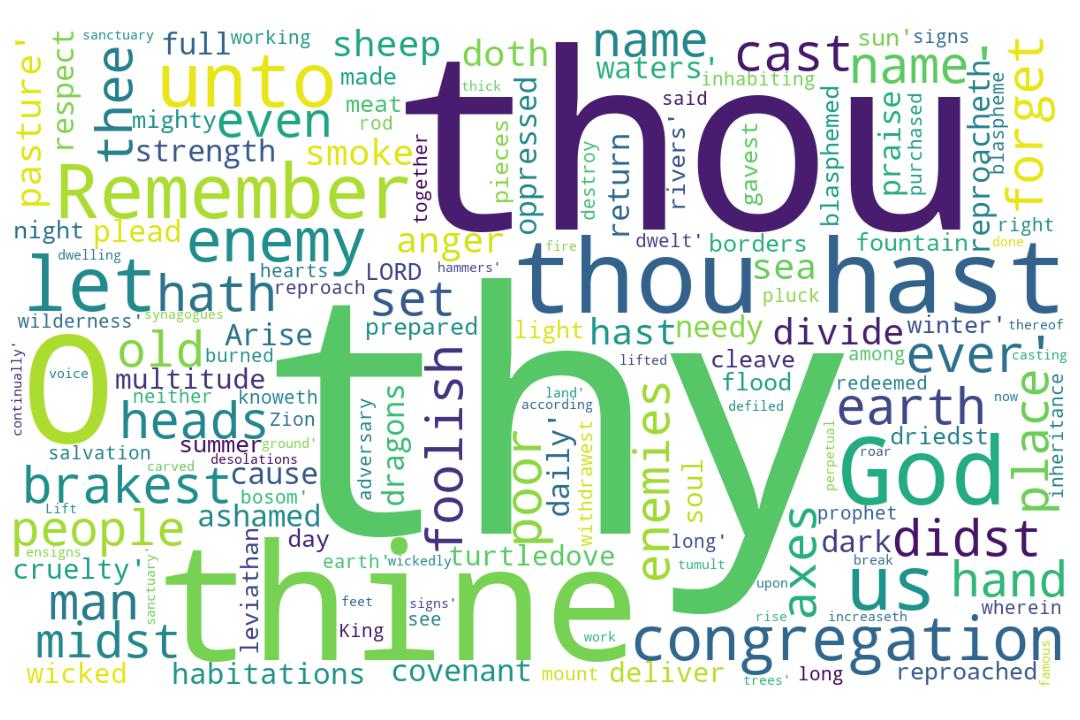
\includegraphics[width=\linewidth]{19OT-Psalms/Psalm74-WordCloud.jpg}
  \caption{Psalm 74 Word Cloud}
  \label{fig:Psalm 74 word Cloud}
\end{figure}


\marginpar{\scriptsize \centering \fcolorbox{bone}{lime}{\textbf{TIMES OF THE GENTILES OVER}}\\ (Psalm 74:1-23) \begin{compactenum}[I.][8]
    \item The \textbf{Smoke} of God's Passion \index[scripture]{Psalms!Psa 074:01}(Psa 74:1)
    \item The \textbf{Sheep} of God's Pasture \index[scripture]{Psalms!Psa 074:01}(Psa 74:1)
    \item The \textbf{Sanctuary} Polluted \index[scripture]{Psalms!Psa 074:03}(Psa 74:3)
    \item The \textbf{Signs} for the People \index[scripture]{Psalms!Psa 074:04}(Psa 74:4)
    \item God's \textbf{Strength}  \index[scripture]{Psalms!Psa 074:13}(Psa 74:13)
   \item \textbf{Supply}  Provided \index[scripture]{Psalms!Psa 074:14}(Psa 74:14)
   \item \textbf{Souls}  Protected \index[scripture]{Psalms!Psa 074:19}(Psa 74:19)
\end{compactenum}}
    



\footnote{\textcolor[cmyk]{0.99998,1,0,0}{\hyperlink{TOC}{Return to end of Table of Contents.}}}\footnote{\href{https://audiobible.com/bible/psalms_74.html}{\textcolor[cmyk]{0.99998,1,0,0}{Psalm 74 Audio}}}\textcolor[cmyk]{0.99998,1,0,0}{Maschil of Asaph}\\
\\
\textcolor[cmyk]{0.99998,1,0,0}{O God, why hast thou cast \emph{us} off for ever? \emph{why} doth thine anger \fcolorbox{bone}{lime}{smoke} against the \fcolorbox{bone}{lime}{sheep} of thy pasture?}\footnote{\textbf{Lamentations 5:20-22} - Wherefore dost thou forget us for ever, and forsake us so long time? [21] Turn thou us unto thee, O LORD, and we shall be turned; renew our days as of old. [22] But thou hast utterly rejected us; thou art very wroth against us.}\footnote{\textbf{Joel 2:32} - And it shall come to pass, that whosoever shall call on the name of the LORD shall be delivered: for in mount Zion and in Jerusalem shall be deliverance, as the LORD hath said, and in the remnant whom the LORD shall call.}\footnote{\textbf{Romans 11:2} - God hath not cast away his people which he foreknew. Wot ye not what the scripture saith of Elias? how he maketh intercession to God against Israel, saying,}\footnote{\textbf{Romans 11:26} - And so all Israel shall be saved: as it is written, There shall come out of Sion the Deliverer, and shall turn away ungodliness from Jacob:}
[2] \textcolor[cmyk]{0.99998,1,0,0}{Remember thy congregation, \emph{which} thou hast purchased of old; the rod of thine inheritance, \emph{which} thou hast redeemed; this mount Zion, wherein thou hast dwelt.}
[3] \textcolor[cmyk]{0.99998,1,0,0}{Lift up thy feet unto the perpetual desolations; \emph{even} all \emph{that} the enemy hath done wickedly in the \fcolorbox{bone}{lime}{sanctuary}.}\footnote{\textbf{Isaiah 63:18} - The people of thy holiness have possessed it but a little while: our adversaries have trodden down thy sanctuary.}\footnote{\textbf{Jeremiah 25:9, 12} - Behold, I will send and take all the families of the north, saith the LORD, and Nebuchadrezzar the king of Babylon, my servant, and will bring them against this land, and against the inhabitants thereof, and against all these nations round about, and will utterly destroy them, and make them an astonishment, and an hissing, and perpetual desolations. [12] And it shall come to pass, when seventy years are accomplished, that I will punish the king of Babylon, and that nation, saith the LORD, for their iniquity, and the land of the Chaldeans, and will make it perpetual desolations.}\footnote{\textbf{Ezekiel 35:9} - I will make thee perpetual desolations, and thy cities shall not return: and ye shall know that I am the LORD.}
[4] \textcolor[cmyk]{0.99998,1,0,0}{Thine enemies roar in the midst of thy \fcolorbox{bone}{MYGOLD}{congregations}; they set up their ensigns \emph{for} \fcolorbox{bone}{lime}{signs}.}
[5] \textcolor[cmyk]{0.99998,1,0,0}{\emph{A} \emph{man} was famous according as he had lifted up axes upon the thick trees.}
[6] \textcolor[cmyk]{0.99998,1,0,0}{But now they break down the carved work thereof at once with axes and hammers.}
[7] \textcolor[cmyk]{0.99998,1,0,0}{They have cast fire into thy sanctuary, they have defiled \emph{by} \emph{casting} \emph{down} the dwelling place of thy name to the ground.}
[8] \textcolor[cmyk]{0.99998,1,0,0}{They said in their hearts, Let us destroy them together: they have burned up all the synagogues of God in the land.}
[9] \textcolor[cmyk]{0.99998,1,0,0}{We see not our signs: \emph{there} \emph{is} no more any prophet: neither \emph{is} \emph{there} among us any that knoweth how long.}
[10] \textcolor[cmyk]{0.99998,1,0,0}{O God, how long shall the adversary reproach? shall the enemy blaspheme thy name for ever?}
[11] \textcolor[cmyk]{0.99998,1,0,0}{Why withdrawest thou thy hand, even thy right hand? pluck \emph{it} out of thy bosom.}
[12] \textcolor[cmyk]{0.99998,1,0,0}{For God \emph{is} my King of old, working salvation in the midst of the earth.}
[13] \textcolor[cmyk]{0.99998,1,0,0}{Thou didst divide the sea by thy \fcolorbox{bone}{lime}{strength}: thou brakest the heads of the dragons in the waters.}
[14] \textcolor[cmyk]{0.99998,1,0,0}{Thou brakest the heads of leviathan in pieces, \emph{and} gavest him \emph{to} \emph{be} \fcolorbox{bone}{lime}{meat} to the people inhabiting the wilderness.}
[15] \textcolor[cmyk]{0.99998,1,0,0}{Thou didst cleave the fountain and the flood: thou driedst up mighty rivers.}
[16] \textcolor[cmyk]{0.99998,1,0,0}{The day \emph{is} thine, the night also \emph{is} thine: thou hast prepared the light and the sun.}
[17] \textcolor[cmyk]{0.99998,1,0,0}{Thou hast set all the borders of the earth: thou hast made summer and winter.}
[18] \textcolor[cmyk]{0.99998,1,0,0}{Remember this, \emph{that} the enemy hath reproached, O LORD, and \emph{that} the foolish people have blasphemed thy name.}
[19] \textcolor[cmyk]{0.99998,1,0,0}{O deliver not the \fcolorbox{bone}{lime}{soul} of thy turtledove unto the multitude \emph{of} \emph{the} \emph{wicked}: forget not the congregation of thy poor for ever.}
[20] \textcolor[cmyk]{0.99998,1,0,0}{Have respect unto the covenant: for the dark places of the earth are full of the habitations of cruelty.}
[21] \textcolor[cmyk]{0.99998,1,0,0}{O let not the oppressed return ashamed: let the poor and needy praise thy name.}
[22] \textcolor[cmyk]{0.99998,1,0,0}{Arise, O God, plead thine own cause: remember how the foolish man reproacheth thee daily.}
[23] \textcolor[cmyk]{0.99998,1,0,0}{Forget not the voice of thine enemies: the tumult of those that rise up against thee increaseth continually.}




